\documentclass[12pt]{article}

%Page Size
\usepackage{geometry}
\geometry{a4paper}

\usepackage{amsmath, mathtools}
\usepackage{amsfonts}
\usepackage{amssymb}
\usepackage{graphicx}
\usepackage{colortbl}
\usepackage{xr}
\usepackage{hyperref}
\usepackage{longtable}
\usepackage{xfrac}
\usepackage{tabularx}
\usepackage{float}
\usepackage{siunitx}
\usepackage{booktabs}
\usepackage{caption}
\usepackage{pdflscape}
\usepackage{afterpage}

%\usepackage[round]{natbib}

%\usepackage{refcheck}

\hypersetup{
    %bookmarks=true,         % show bookmarks bar?
      colorlinks=true,       % false: boxed links; true: colored links
    linkcolor=red,          % color of internal links (change box color with linkbordercolor)
    citecolor=green,        % color of links to bibliography
    filecolor=magenta,      % color of file links
    urlcolor=cyan           % color of external links
}

% Include common files
\input{../Comments}
%% Common Parts

\newcommand{\progname}{Cut Edge Weight: Data Separability Measurement} % PUT YOUR PROGRAM NAME HERE
\newcommand{\authname}{Lesley Wheat} % AUTHOR NAMES                  

\usepackage{hyperref}
    \hypersetup{colorlinks=true, linkcolor=blue, citecolor=blue, filecolor=blue,
                urlcolor=blue, unicode=false}
    \urlstyle{same}
                                



% For easy change of table widths
\newcommand{\colZwidth}{1.0\textwidth}
\newcommand{\colAwidth}{0.13\textwidth}
\newcommand{\colBwidth}{0.82\textwidth}
\newcommand{\colCwidth}{0.1\textwidth}
\newcommand{\colDwidth}{0.05\textwidth}
\newcommand{\colEwidth}{0.8\textwidth}
\newcommand{\colFwidth}{0.17\textwidth}
\newcommand{\colGwidth}{0.5\textwidth}
\newcommand{\colHwidth}{0.28\textwidth}

% Used so that cross-references have a meaningful prefix
\newcounter{defnum} %Definition Number
\newcommand{\dthedefnum}{GD\thedefnum}
\newcommand{\dref}[1]{GD\ref{#1}}
\newcounter{datadefnum} %Datadefinition Number
\newcommand{\ddthedatadefnum}{DD\thedatadefnum}
\newcommand{\ddref}[1]{DD\ref{#1}}
\newcounter{theorynum} %Theory Number
\newcommand{\tthetheorynum}{T\thetheorynum}
\newcommand{\tref}[1]{T\ref{#1}}
\newcounter{tablenum} %Table Number
\newcommand{\tbthetablenum}{T\thetablenum}
\newcommand{\tbref}[1]{TB\ref{#1}}
\newcounter{assumpnum} %Assumption Number
\newcommand{\atheassumpnum}{P\theassumpnum}
\newcommand{\aref}[1]{A\ref{#1}}
\newcounter{goalnum} %Goal Number
\newcommand{\gthegoalnum}{P\thegoalnum}
\newcommand{\gsref}[1]{GS\ref{#1}}
\newcounter{instnum} %Instance Number
\newcommand{\itheinstnum}{IM\theinstnum}
\newcommand{\iref}[1]{IM\ref{#1}}
\newcounter{reqnum} %Requirement Number
\newcommand{\rthereqnum}{P\thereqnum}
\newcommand{\rref}[1]{R\ref{#1}}
\newcounter{nfrnum} %NFR Number
\newcommand{\rthenfrnum}{NFR\thenfrnum}
\newcommand{\nfrref}[1]{NFR\ref{#1}}
\newcounter{lcnum} %Likely change number
\newcommand{\lthelcnum}{LC\thelcnum}
\newcommand{\lcref}[1]{LC\ref{#1}}

\usepackage{fullpage}

\newcommand{\deftheory}[9][Not Applicable]
{
\newpage
\noindent \rule{\textwidth}{0.5mm}

\paragraph{RefName: } \textbf{#2} \phantomsection 
\label{#2}

\paragraph{Label:} #3

\noindent \rule{\textwidth}{0.5mm}

\paragraph{Equation:}

#4

\paragraph{Description:}

#5

\paragraph{Notes:}

#6

\paragraph{Source:}

#7

\paragraph{Ref.\ By:}

#8

\paragraph{Preconditions for \hyperref[#2]{#2}:}
\label{#2_precond}

#9

\paragraph{Derivation for \hyperref[#2]{#2}:}
\label{#2_deriv}

#1

\noindent \rule{\textwidth}{0.5mm}

}

\begin{document}

\title{Software Requirements Specification for \progname: Data Separability Measurement} 
\author{\authname}
\date{\today}
	
\maketitle

~\newpage

\pagenumbering{roman}

\tableofcontents

~\newpage

\section*{Revision History}

\begin{tabularx}{\textwidth}{p{3cm}p{2cm}X}
\toprule {\bf Date} & {\bf Version} & {\bf Notes}\\
\midrule
2023-01-24 & 0.0 & Creation \\
2023-02-01 & 0.1 & Revise Instance Models \\
2023-02-03 & 1.0 & Version 1 Release \\
\bottomrule
\end{tabularx}

~\newpage

\section{Reference Material}

This section records information for easy reference.

\subsection{Table of Units}

Throughout this document no units are used.

\subsection{Table of Symbols}

The table that follows summarizes the symbols used in this document along with their units.  
The choice of symbols was made to be consistent with the statistics literature.

\renewcommand{\arraystretch}{1.2}
%\noindent \begin{tabularx}{1.0\textwidth}{l l X}
\noindent \begin{longtable*}{l l p{12cm}} \toprule
\textbf{Symbol} & \textbf{Unit} & \textbf{Description}\\
\midrule 
$I(...)$ & N/A & Indicator Function \\ %Ellipsis
$J_N$ & N/A & Normalized Multiclass Cut Edge Weight Measurement \\
\bottomrule
\end{longtable*}
\mycomment{Use your problems actual symbols.  The si package is a good idea to use for
  units.}

\subsection{Abbreviations and Acronyms}

\renewcommand{\arraystretch}{1.2}
\begin{tabular}{l l} 
  \toprule		
  \textbf{Symbol} & \textbf{Description}\\
  \midrule 
  A & Assumption\\
  CEWS & Cut Edge Weight Statistic\\
  DD & Data Definition\\
  GD & General Definition\\
  GS & Goal Statement\\
  IM & Instance Model\\
  LC & Likely Change\\
  PS & Physical System Description\\
  R & Requirement\\
  RNG & Relative Neighbourhood Graph\\
  SRS & Software Requirements Specification\\
  T & Theoretical Model\\
  \bottomrule
\end{tabular}\\

\subsection{Mathematical Notation}

This document uses notation used in \cite{zighed_statistical_2005}.

\mycomment{This section is optional, but should be included for projects that make use of notation to convey mathematical information.  
For instance, if typographic conventions (like bold face font) are used to distinguish matrices, this should be stated here.  
If symbols are used to show mathematical operations, these should be summarized here.  
In some cases the easiest way to summarize the notation is to point to a text or other source that explains the notation.}

\mycomment{This section was added to the template because some students use very
  domain specific notation.  This notation will not be readily understandable to
  people outside of your domain.  It should be explained.}

\newpage

\pagenumbering{arabic}

\mycomment{This SRS template is based on \citet{SmithAndLai2005, SmithEtAl2007}.  It
  will get you started.  You should not modify the section headings, without
  first discussing the change with the course instructor.  Modification means
  you are not following the template, which loses some of the advantage of a
  template, especially standardization.  Although the bits shown below do not
  include type information, you may need to add this information for your
  problem.  If you are unsure, please can ask the instructor.}

\mycomment{Feel free to change the appearance of the report by modifying the LaTeX
  commands.}

\mycomment{This template document assumes that a single program is being documented.
  If you are documenting a family of models, you should start with a commonality
  analysis.  A separate template is provided for this.  For program
  families you should look at \cite{Smith2006, SmithMcCutchanAndCarette2017}.
  Single family member programs are often programs based on a single physical
  model.  General purpose tools are usually documented as a family.  Families of
  physical models also come up.}

\mycomment{The SRS is not generally written, or read, sequentially.  The SRS is a
  reference document.  It is generally read in an ad hoc order, as the need
  arises.  For writing an SRS, and for reading one for the first time, the
  suggested order of sections is:
\begin{itemize}
\item Goal Statement
\item Instance Models
\item Requirements
\item Introduction
\item Specific System Description
\end{itemize}
}

\mycomment{Guiding principles for the SRS document:
\begin{itemize}
\item Do not repeat the same information at the same abstraction level.  If
  information is repeated, the repetition should be at a different abstraction
  level.  For instance, there will be overlap between the scope section and the
  assumptions, but the scope section will not go into as much detail as the
  assumptions section.
\end{itemize}
}

\mycomment{The template description comments should be disabled before submitting this
  document for grading.}

\mycomment{You can borrow any wording from the text given in the template.  It is part
  of the template, and not considered an instance of academic integrity.  Of
  course, you need to cite the source of the template.}

\mycomment{When the documentation is done, it should be possible to trace back to the
  source of every piece of information.  Some information will come from
  external sources, like terminology.  Other information will be derived, like
  General Definitions.}

\mycomment{An SRS document should have the following qualities: unambiguous,
  consistent, complete, validatable, abstract and traceable.}

\mycomment{The overall goal of the SRS is that someone that meets the Characteristics
  of the Intended Reader (Section~\ref{sec:IntendedReader}) can learn,
  understand and verify the captured domain knowledge.  They should not have to
  trust the authors of the SRS on any statements.  They should be able to
  independently verify/derive every statement made.}

\section{Introduction}

Classification is a common machine learning problem and there are many techniques for solving classification problems. 
Unfortunately, not all classification problems are easy and it can be difficult to explain why classifiers preform poorly on certain datasets. 
Data complexity has been defined as a characteristic of the data that relates to the difficulty of the classification problem \cite{luengo_automatic_2015}. 
To further refine this definition, we consider data complexity to be represented by aspects of the data that introduce difficulty for the classifiers. 

One of these aspects is separability, an intrinsic characteristic that describes how the data points from different classes mix together \cite{guan_novel_2021}. 
A classic measurement for separability is Fraction of Points on Class Boundary.
Based on the work of Friedman and Rafsky \cite{friedman_multivariate_1979} and documented by Basu and Ho\cite{ho_complexity_2002}, this measurement constructs a minimum spanning tree over the dataset then calculates the number of points with a connection to another class over all points.

The Cut Edge Weight Statistic measurement \cite{zighed_statistical_2005} is a variation of the Fraction of Points on Class Boundary, proposed by Zighed et al. 
The algorithm for the normalized measurement begins by constructing a Toussaint’s Relative Neighbourhood Graph \cite{toussaint_relative_1980} over the entire dataset then computing the number of edges which connect different classes (the "cut edges") over the total number of edges. 
This measurement is a viable way of measuring separability because it has a high coefficient of determination ($R^2$) with the mean error rate of several classifiers.

\begin{figure}[h!]
\begin{center}
 \includegraphics[width=0.7\textwidth]{RNG_CEWS_Example.png}
\caption{An visualization of the RNG for a binary classification problem represented by black and white points. (a) An example of a 2D RNG graph construction. (b) Identifying cut edges with dotted lines.}
\label{Fig_RNG} 
\end{center}
\end{figure}

The introduction contains the purpose of this document, the scope of requirements, characteristics of the indented reader and the organization of this complete
document.

\mycomment{The introduction section is written to introduce the problem.  It starts
  general and focuses on the problem domain. The general advice is to start with
a paragraph or two that describes the problem, followed by a ``roadmap''
paragraph.  A roadmap orients the reader by telling them what sub-sections to
expect in the Introduction section.}

\subsection{Purpose of Document}

The purpose of this document is to provide information about the design and functionality of CEWS System to the Intended Reader (Section \ref{sec:IntendedReader}).

\mycomment{This section summarizes the purpose of the SRS document.  It does not focus
  on the problem itself.  The problem is described in the ``Problem
  Description'' section (Section~\ref{sec:pd}).  The purpose is for the document
  in the context of the project itself, not in the context of this course.
  Although the ``purpose'' of the document is to get a grade, you should not
  mention this.  Instead, ``fake it'' as if this is a real project.  The purpose
  section will be similar between projects.  The purpose of the document is the
  purpose of the SRS, including communication, planning for the design stage,
  etc.}

\subsection{Scope of Requirements} 

The domain of this problem is restricted to generating the normalized multiclass CEWS Measurement \cite{zighed_statistical_2005}. Notable exclusions include the calculation of a p-value, variations of the calculation using different weighing parameters and different graph generation algorithms. The scope excludes asymptotic cost limitations and efficiency requirements. 

\mycomment{Modelling the real world requires simplification.  The full complexity of
  the actual physics, chemistry, biology is too much for existing models, and
  for existing computational solution techniques.  Rather than say what is in
  the scope, it is usually easier to say what is not.  You can think of it as
  the scope is initially everything, and then it is constrained to create the
  actual scope.  For instance, the problem can be restricted to 2 dimensions, or
  it can ignore the effect of temperature (or pressure) on the material
  properties, etc.}  

\mycomment{The scope section is related to the assumptions section
  (Section~\ref{sec:assumpt}).  However, the scope and the assumptions are not
  at the same level of abstraction.  The scope is at a high level.  The focus is
  on the ``big picture'' assumptions.  The assumptions section lists, and
  describes, all of the assumptions.}

\subsection{Characteristics of Intended Reader} \label{sec:IntendedReader}

The reader should have a good understanding of classification (at a graduate level or equivalent experience). The reader should have a base understanding of data analysis, machine learning and statistics such as from standard undergraduate courses.

\mycomment{This section summarizes the skills and knowledge of the readers of the SRS.  
It does NOT have the same purpose as the ``User Characteristics'' section (Section~\ref{sec:UserCharacteristics}).  
The intended readers are the people that will read, review and maintain the SRS.  
They are the people that will conceivably design the software that is intended to meet the requirements.  
The user, on the other hand, is the person that uses the software that is built.  
They may never read this SRS document.  Of course, the same person could be a ``user'' and an ``intended reader.''}

\mycomment{The intended reader characteristics should be written as unambiguously and as specifically as possible.  Rather than say, the user should have an
  understanding of physics, say what kind of physics and at what level.  For
  instance, is high school physics adequate, or should the reader have had a
  graduate course on advanced quantum mechanics?}

\subsection{Organization of Document}

This document includes a general system description, a specific system description, a requirements section, a section on likely changes, a section on unlikely changes and a section on traceability.

\mycomment{This section provides a roadmap of the SRS document. 
It will help the reader orient themselves.  
It will provide direction that will help them select which sections they want to read, and in what order.
This section will be similar between project.}

\section{General System Description}

This section provides general information about the system.  
It identifies the interfaces between the system and its environment, describes the user characteristics and lists the system constraints. 

\mycomment{The purpose of this section is to provide general information about the
  system so the specific requirements in the next section will be easier to
  understand. The general system description section is designed to be
  changeable independent of changes to the functional requirements documented in
  the specific system description. The general system description provides a
  context for a family of related models.  The general description can stay the
  same, while specific details are changed between family members.}

\subsection{System Context}

The CEWS System will exist as a standalone product or as a module. The system context is illustrated in Figure \ref{Fig_SystemContext}. 

\mycomment{Your system context will include a figure that shows the abstract view of
  the software.  Often in a scientific context, the program can be viewed
  abstractly following the design pattern of Inputs $\rightarrow$ Calculations
  $\rightarrow$ Outputs.  The system context will therefore often follow this
  pattern.  The user provides inputs, the system does the calculations, and then
  provides the outputs to the user.  The figure should not show all of the
  inputs, just an abstract view of the main categories of inputs (like material
  properties, geometry, etc.).  Likewise, the outputs should be presented from
  an abstract point of view.  In some cases the diagram will show other external
  entities, besides the user.  For instance, when the software product is a
  library, the user will be another software program, not an actual end user.
  If there are system constraints that the software must work with external
  libraries, these libraries can also be shown on the System Context diagram.
  They should only be named with a specific library name if this is required by
  the system constraint.}

\begin{figure}[h!]
\begin{center}
 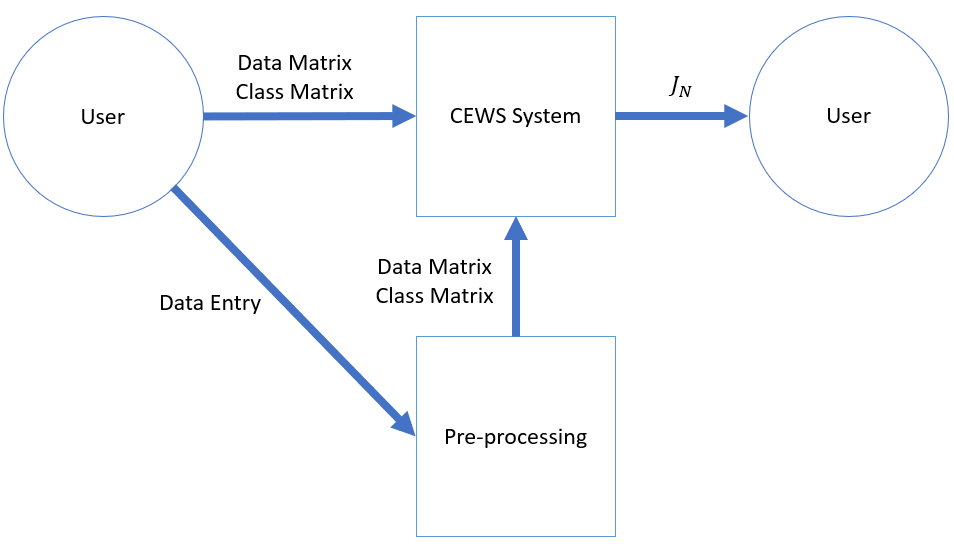
\includegraphics[width=0.7\textwidth]{SystemContext_2.png}
\caption{System Context}
\label{Fig_SystemContext} 
\end{center}
\end{figure}

\mycomment{For each of the entities in the system context diagram its responsibilities
  should be listed.  Whenever possible the system should check for data quality,
  but for some cases the user will need to assume that responsibility.  The list
  of responsibilites should be about the inputs and outputs only, and they
  should be abstract.  Details should not be presented here.  However, the
  information should not be so abstract as to just say ``inputs'' and
  ``outputs''.  A summarizing phrase can be used to characterize the inputs.
  For instance, saying ``material properties'' provides some information, but it
  stays away from the detail of listing every required properties.}


\begin{itemize}
\begin{samepage}
\item User Responsibilities:
\begin{itemize}
\item Provide the data.
\item Correctly format the input data matrices as per Section \ref{sec:dataConstraints}.
\item Resource management including supplying the system with enough resources to support the size of their dataset.
\item Understand the problem.
\item Preform any data pre-processing required for the relevant classification problem such as transformations, feature extraction, etc.
\item Understand the CEWS algorithm.
\item Understand the limitations of numerical computation. 
\end{itemize}
\end{samepage}

\begin{samepage}
\item \progname{} Responsibilities:
\begin{itemize}
\item Read input data.
\item Detect data type mismatch or if input data violates any constraints.
\item Preform the analysis.
\item Preform basic error checking on the output.
\item Return the output value.
\end{itemize}
\end{samepage}
\end{itemize}

\subsection{User Characteristics} \label{sec:UserCharacteristics}

The end user of CEWS System should have a good understanding of classification and machine learning, preferably with an undergraduate degree in software or math.

\mycomment{This section summarizes the knowledge/skills expected of the user.
Measuring usability, which is often a required non-function requirement, requires knowledge of a typical user.  
As mentioned above, the user is a different role from the ``intended reader,'' as given in Section~\ref{sec:IntendedReader}.
As in Section~\ref{sec:IntendedReader}, the user characteristics should be specific an unambiguous.  For instance, ``The end user of \progname{} should have an understanding of undergraduate Level 1 Calculus and Physics.''}

\subsection{System Constraints}

At this time, there are no known constraints for this system..

\mycomment{System constraints differ from other type of requirements because they limit the developers' options in the system design and they identify how the eventual system must fit into the world.
This is the only place in the SRS where design decisions can be specified. 
That is, the quality requirement for abstraction is relaxed here.
However, system constraints should only be included if they are truly required.}

\section{Specific System Description}

This section first presents the problem description, which gives a high-level
view of the problem to be solved.  This is followed by the solution characteristics
specification, which presents the assumptions, theories, definitions and finally
the instance models.  \mycomment{Add any project specific details that are relevant
  for the section overview.}

\subsection{Problem Description} \label{sec:pd}

\progname{} is intended to solve the calculation of the normalized multiclass CEWS measurement for a dataset. \mycomment{What problem does your program solve?
The description here should be in the problem space, not the solution space.}

\subsubsection{Terminology and  Definitions}

\mycomment{This section is expressed in words, not with equations.  It provide the
  meaning of the different words and phrases used in the domain of the problem.
The terminology is used to introduce concepts from the world outside of the
mathematical model  The terminology provides a real world connection to give the
mathematical model meaning.}

This subsection provides a list of terms that are used in the subsequent
sections and their meaning, with the purpose of reducing ambiguity and making it
easier to correctly understand the requirements:

\begin{itemize}
\item Data point/Example/Samples: An identifiable element in a data set which has features associated with it.
\item Data set: A set of examples from a population.
\item Feature : An individual measurable property of an example.
\item Class Label : Represents the class an example belongs to.
\item Classification: The problem of identifying which of a set of categories an example belongs to.
\item Data complexity: Aspects of the data that classifiers have difficultly with. \cite{luengo_automatic_2015}
\item Separability: An intrinsic characteristic of a dataset and describes how the data points from different classes mix together. \cite{guan_novel_2021}
\item Boolean variable : A variable that has one of two possible values.
\end{itemize}

\subsubsection{Physical System Description} \label{sec:phySystDescrip}

There is no physical system.

\mycomment{The purpose of this section is to clearly and unambiguously state the
  physical system that is to be modelled. Effective problem solving requires a
  logical and organized approach. The statements on the physical system to be
  studied should cover enough information to solve the problem. The physical
  description involves element identification, where elements are defined as
  independent and separable items of the physical system. Some example elements
  include acceleration due to gravity, the mass of an object, and the size and
  shape of an object. Each element should be identified and labelled, with their
  interesting properties specified clearly. The physical description can also
  include interactions of the elements, such as the following: i) the
  interactions between the elements and their physical environment; ii) the
  interactions between elements; and, iii) the initial or boundary conditions.

The physical system of \progname{}, as shown in Figure~?, includes the following elements:

\begin{itemize}

\item[PS1:] 

\item[PS2:] ...

\end{itemize}
}


\subsubsection{Goal Statements}

\mycomment{The goal statements refine the ``Problem Description''
  (Section~\ref{sec:pd}).  A goal is a functional objective the system under
  consideration should achieve. Goals provide criteria for sufficient
  completeness of a requirements specification and for requirements
  pertinence. Goals will be refined in Section “Instanced Models”
  (Section~\ref{sec:instance}). Large and complex goals should be decomposed
  into smaller sub-goals.  The goals are written abstractly, with a minimal
  amount of technical language.  They should be understandable by non-domain
  experts.}

\noindent Given the dataset, the goal statements are:

\begin{itemize}

\item[GS\refstepcounter{goalnum}\thegoalnum \label{G:CEWS}:]  Calculate the normalized multiclass CEWS measurement. \mycomment{One
    sentence description of the goal.  There may be more than one.  Each Goal
    should have a meaningful label.}

\end{itemize}

\subsection{Solution Characteristics Specification}

\mycomment{This section specifies the information in the solution domain of the system
  to be developed. This section is intended to express what is required in
  such a way that analysts and stakeholders get a clear picture, and the
  latter will accept it. The purpose of this section is to reduce the problem
  into one expressed in mathematical terms. Mathematical expertise is used to
  extract the essentials from the underlying physical description of the
  problem, and to collect and substantiate all physical data pertinent to the
  problem.}

\mycomment{This section presents the solution characteristics by successively refining
  models.  It starts with the abstract/general Theoretical Models (TMs) and
  refines them to the concrete/specific Instance Models (IMs).  If necessary
  there are intermediate refinements to General Definitions (GDs).  All of these
  refinements can potentially use Assumptions (A) and Data Definitions (DD).
  TMs are refined to create new models, that are called GMs or IMs. DDs are not
  refined; they are just used. GDs and IMs are derived, or refined, from other
  models. DDs are not derived; they are just given. TMs are also just given, but
  they are refined, not used.  If a potential DD includes a derivation, then
  that means it is refining other models, which would make it a GD or an IM.}

\mycomment{The above makes a distinction between ``refined'' and ``used.'' A model is
  refined to another model if it is changed by the refinement. When we change a
  general 3D equation to a 2D equation, we are making a refinement, by applying
  the assumption that the third dimension does not matter. If we use a
  definition, like the definition of density, we aren't refining, or changing
  that definition, we are just using it.}

\mycomment{The same information can be a TM in one problem and a DD in another.  It is
  about how the information is used.  In one problem the definition of
  acceleration can be a TM, in another it would be a DD.}

\mycomment{There is repetition between the information given in the different chunks
  (TM, GDs etc) with other information in the document.  For instance, the
  meaning of the symbols, the units etc are repeated.  This is so that the
  chunks can stand on their own when being read by a reviewer/user.  It also
  facilitates reuse of the models in a different context.}

\noindent \mycomment{The relationships between the parts of the document are show in
  the following figure.  In this diagram ``may ref'' has the same role as
  ``uses'' above.  The figure adds ``Likely Changes,'' which are able to
  reference (use) Assumptions.}

%\begin{figure}[H]
  %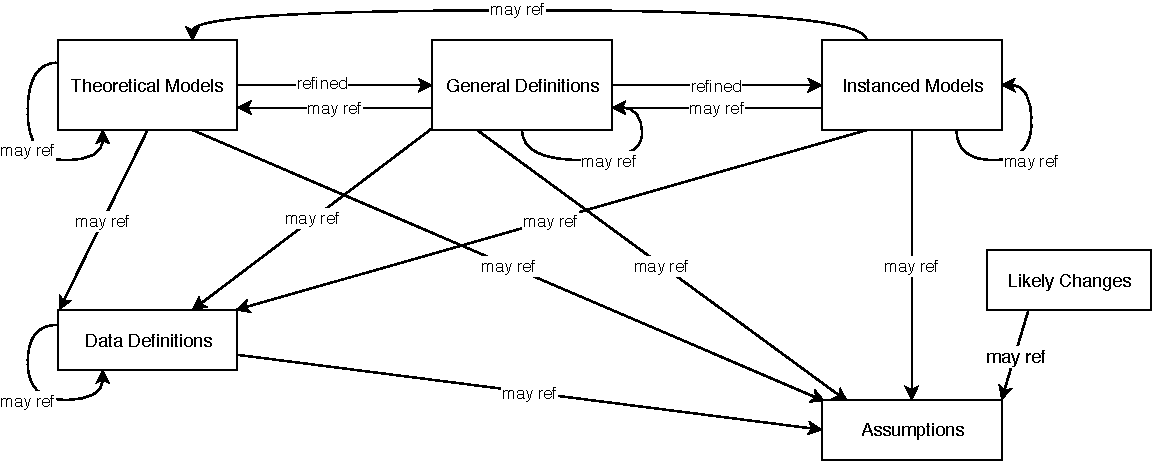
\includegraphics[scale=0.9]{RelationsBetweenTM_GD_IM_DD_A.pdf}
%\end{figure}

The instance models that govern \progname{} are presented in
Subsection~\ref{sec:instance}.  The information to understand the meaning of the
instance models and their derivation is also presented, so that the instance
models can be verified.

\subsubsection{Assumptions} \label{sec:assumpt}

\mycomment{The assumptions are a refinement of the scope.  The scope is general, where
  the assumptions are specific.  All assumptions should be listed, even those
  that domain experts know so well that they are rarely (if ever) written down.}
\mycomment{The document should not take for granted that the reader knows which
  assumptions have been made. In the case of unusual assumptions, it is
  recommended that the documentation either include, or point to, an explanation
  and justification for the assumption.}

This section simplifies the original problem and helps in developing the
theoretical model by filling in the missing information for the physical
system. The numbers given in the square brackets refer to the theoretical model
[T], general definition [GD], data definition [DD], instance model [IM], or
likely change [LC], in which the respective assumption is used.

\begin{itemize}

\item[A\refstepcounter{assumpnum}\theassumpnum \label{A:fp}:]
All rational numbers can be represented in a base 2 computer system. Operations preformed on rational numbers in a computer system is exact. Any computation rounding error is negligible and does not need to be taken into account.

\item[A\refstepcounter{assumpnum}\theassumpnum \label{A:CWN}:]
Class labels are represented as whole numbers. All examples from one class share the same class label.

\item[A\refstepcounter{assumpnum}\theassumpnum \label{A:NOF}:]
Each example has the same number of features. No features are null. 

\item[A\refstepcounter{assumpnum}\theassumpnum \label{A:weights}:]
The user does not want to use weights for the edge calculation.

\item[A\refstepcounter{assumpnum}\theassumpnum \label{A:rng}:]
The user wants to use a relative neighbourhood graph as the base graph.

\item[A\refstepcounter{assumpnum}\theassumpnum \label{A:pvalue}:]
The user doesn't want the statistic p-value.

  \mycomment{Short description of each assumption.  Each assumption
    should have a meaningful label.  Use cross-references to identify the
    appropriate traceability to T, GD, DD etc., using commands like dref, ddref
    etc.  Each assumption should be atomic - that is, there should not be an
    explicit (or implicit) ``and'' in the text of an assumption.}

\end{itemize}

\subsubsection{Theoretical Models}\label{sec:theoretical}

No theoretical models are used.

\mycomment{
\mycomment{Theoretical models are sets of abstract mathematical equations or axioms
  for solving the problem described in Section ``Physical System Description''
  (Section~\ref{sec:phySystDescrip}). Examples of theoretical models are
  physical laws, constitutive equations, relevant conversion factors, etc.}

This section focuses on the general equations and laws that \progname{} is based
on.  \mycomment{Modify the examples below for your problem, and add additional models
  as appropriate.}

~\newline

\noindent
\deftheory
% #2 refname of theory
{T:SCE}
% #3 label
{Sum of Cut Edges}
% #4 equation
{\\
J = \sum_{r=1}^{k-1} \sum_{s=r+1}^{k} J_{r,s} =  \frac {1}{2} \sum_{2}^{} Z_{ij} \\
}
% #5 description
{
The above equations give the formula for calculating the multiclass is the sum of cut edges where $k$ is the number of classes, $Z_{ij}$ is a boolean variable indicating different classes (one if the vertices $i$ and $j$ have different and zero if not) and $J_{r,s}$ is the sum of edges linking a vertex of class $r$ and a vertex of class $s$.

}
% #6 Notes
{
None.
}
% #7 Source
{
  \cite{zighed_statistical_2005}
}
% #8 Referenced by
{
  %\dref{ROCT}
}
% #9 Preconditions
{
None
}
% #1 derivation - not applicable by default
{}

\mycomment{``Ref.\ By'' is used repeatedly with the different types of information.
  This stands for Referenced By.  It means that the models, definitions and
  assumptions listed reference the current model, definition or assumption.
  This information is given for traceability.  Ref. By provides a pointer in the
  opposite direction to what we commonly do.  You still need to have a reference
  in the other direction pointing to the current model, definition or
  assumption.  As an example, if T1 is referenced by G2, that means that G2 will
  explicitly include a reference to T1.}

~\newline

\noindent
\deftheory
% #2 refname of theory
{T:SNCE}
% #3 label
{Sum of Non Cut Edges}
% #4 equation
{\\
I = \sum_{r=1}^{k} I_r = \frac {1}{2} \sum_{2}^{} T_{ij} \\
}
% #5 description
{
The above equations give the formula for calculating the the multiclass sum of non cut edges, $I_r$ is the sum of weights relative to edges linking two vertices of the same class for class $r$ and $T_{ij}$ is a boolean variable indicating same class (one if the vertices $i$ and $j$ have the classes are the same and zero if not).

}
% #6 Notes
{
None.
}
% #7 Source
{
  \cite{zighed_statistical_2005}
}
% #8 Referenced by
{
  %\dref{ROCT}
}
% #9 Preconditions
{
None
}
% #1 derivation - not applicable by default
{}

~\newline
}
\subsubsection{General Definitions}\label{sec:gendef}

This section collects and equations that will be used in building the
instance models.

% RNG

~\newline
\noindent
\begin{minipage}{\textwidth}
\renewcommand*{\arraystretch}{1.5}
\begin{tabular}{| p{\colAwidth} | p{\colBwidth}|}
\hline
\rowcolor[gray]{0.9}
Number& GD\refstepcounter{defnum}\thedefnum \label{GD:RNG}\\
\hline
Label &\bf Toussaint’s Relative Neighbourhood Graph \\ \hline
SI Units& N/A \\ \hline
Equation & $E_{RNG}(P, i, j) = [ d(p_i,p_j) \leq \max (d(p_i,c), d(p_j,c)) \forall c $ \\
& where $c \in P, c \neq p_i, c \neq p_j ]$\\
& Connection matrix: $V = (v_{ij}), i = 1,2, ... ,n; j = 1,2, ... , n;$ \\
& where $v_{ij} = I(E_{RNG}(P, i, j))$ \\ \hline
Description &
RNG is an undirected graph constructed by connecting an edge between two points when a third point does not exist that is closer to both.\\
& $P$ is a set of $n$ points in real space with dimensions $m$.\\
& $V$ is the connection matrix where $v_{ij} =  1$ if there is an edge and $v_{ij} =  0$ if not.\\
& $d(a,b)$ is the Euclidean distance between points $a$ and $b$ given by \ddref{DD:ED}.\\
\hline
  Source & \cite{zighed_statistical_2005} \\ \hline
  Ref.\ By & \iref{IM:CEWS} \\ \hline
\end{tabular}
\end{minipage}\\

\mycomment{
~\newline
\noindent
\begin{minipage}{\textwidth}
\renewcommand*{\arraystretch}{1.5}
\begin{tabular}{| p{\colAwidth} | p{\colBwidth}|}
\hline
\rowcolor[gray]{0.9}
Number& GD\refstepcounter{defnum}\thedefnum \label{GD:SCE}\\
\hline
Label &\bf Sum of Cut Edges \\ \hline
SI Units& N/A \\ \hline
Equation & $J = \sum_{r=1}^{k-1} \sum_{s=r+1}^{k} J_{r,s} =  \frac {1}{2} \sum_{2}^{} Z_{ij}$  \\ \hline
Description &
The above equation gives the formula for calculating the multiclass is the sum of cut edges.
\\
& $k$ is the number of classes.\\
& $J_{r,s}$ is the sum of edges linking a vertex of class $r$ and a vertex of class $s$ based on \dref{GD:RNG}.\\
& $Z_{ij}$ is a boolean variable indicating different classes (one if the vertices $i$ and $j$ have different and zero if not).\\
\hline
  Source & \cite{zighed_statistical_2005} \\ \hline
  Ref.\ By & \iref{IM:CEWS} \\ \hline
\end{tabular}
\end{minipage}\\

~\newline
\noindent
\begin{minipage}{\textwidth}
\renewcommand*{\arraystretch}{1.5}
\begin{tabular}{| p{\colAwidth} | p{\colBwidth}|}
\hline
\rowcolor[gray]{0.9}
Number& GD\refstepcounter{defnum}\thedefnum \label{GD:SNCE}\\
\hline
Label &\bf Sum of Non Cut Edges \\ \hline
SI Units& N/A \\ \hline
Equation &  $I = \sum_{r=1}^{k} I_r = \frac {1}{2} \sum_{2}^{} T_{ij}$  \\ \hline
Description &
The above equation gives the formula for calculating the the multiclass sum of non cut edges.
\\
& $k$ is the number of classes.\\
& $I_r$ is the sum of edges linking two vertices of the same class for class $r$ based on \dref{GD:RNG}.\\
& $T_{ij}$ is a boolean variable indicating same class (one if the vertices $i$ and $j$ have the classes are the same and zero if not).\\

\hline
  Source & \cite{zighed_statistical_2005} \\ \hline
  Ref.\ By &  \iref{IM:CEWS} \\ \hline
\end{tabular}
\end{minipage}\\
}


\subsubsection{Data Definitions}\label{sec:datadef}

This section collects and defines all the data needed to build the instance
models. The dimension of each quantity is also given. 

~\newline

\noindent
\begin{minipage}{\textwidth}
\renewcommand*{\arraystretch}{1.5}
\begin{tabular}{| p{\colAwidth} | p{\colBwidth}|}
\hline
\rowcolor[gray]{0.9}
Number& DD\refstepcounter{datadefnum}\thedatadefnum \label{DD:ED}\\
\hline
Label& \bf Euclidean distance\\ \hline
Symbol &$d(a,b)$\\ \hline
  SI Units & N/A \\\hline
  Equation & $d(a,b) = \sqrt{\sum^n_{i=1} (a_i - b_i)^2 }$ \\\hline
  Description & 
                $d(a,b)$ is the Euclidiean distance between points $a$ and $b$ in Euclidean space with $n$ dimensions.  
                $a_i$ and $b_i$ are Euclidean vectors from the origin. 
  \\ \hline
  Sources& N/A \\ \hline
  Ref.\ By & \dref{GD:RNG} \\ \hline
\end{tabular}
\end{minipage}\\

\subsubsection{Instance Models} \label{sec:instance}    

\mycomment{The motivation for this section is to reduce the problem defined in
  ``Physical System Description'' (Section~\ref{sec:phySystDescrip}) to one
  expressed in mathematical terms. The IMs are built by refining the TMs and/or
  GDs.  This section should remain abstract.  The SRS should specify the
  requirements without considering the implementation.}

This section transforms the problem defined in Section~\ref{sec:pd} into 
one which is expressed in mathematical terms. It uses concrete symbols defined 
in Section~\ref{sec:datadef} to replace the abstract symbols in the models 
identified in Sections~\ref{sec:theoretical} and~\ref{sec:gendef}.
The goals \mycomment{reference your goals} are solved by \iref{IM:CEWS}, which is the implementation of the cut edge weight statistic measurement.

\mycomment{reference your instance models}  
\mycomment{other details, with cross-references where appropriate.}
\mycomment{Modify the examples below for your problem, and add additional models as
  appropriate.}

~\newline

%CEWS

\noindent
\begin{minipage}{\textwidth}
\renewcommand*{\arraystretch}{1.5}
\begin{tabular}{| p{\colAwidth} | p{\colBwidth}|}
    \hline
    \rowcolor[gray]{0.9}
    Number& IM\refstepcounter{instnum}\theinstnum \label{IM:CEWS}\\
    \hline
    Label& \bf Multiclass Normalized Cut Edge Weight Measurement\\
    \hline
    Input & The input data matrix, $D$, and the class label matrix, $C$, based on \ref{sec:dataConstraints}. \\ \hline
    Output&$J_{N}$, $0\leq J_N \leq 1$, such that\\
    &$J_{N} = \frac {J}{I+J}$\\
    & where \\
    & $J = \sum_{r=1}^{k-1} \sum_{s=r+1}^{k} J_{r,s}; 0 \leq J \leq n^2$\\
    & $J_{r,s}  = \sum^{n}_{i=1} \sum^n_{j=1} V_{ij} \times I(c_i = r \And c_j = s)$ \\
    & $I = \sum_{r=1}^{k} I_r, 0\leq I \leq  n^2$ \\
    & $I_{r}  = \sum^{n-1}_{i=1} \sum^n_{j=i+1} V_{ij} \times I(c_i = r \And c_j = r)$ \\
    \hline
    Description &
    The above equation gives the formula for calculating the the multiclass normalized cut edge weight measurement. \\
    & $k$ is the number of classes.\\
    & $V_{ij}$ is the RNG connection matrix for matrix $D$ given by \dref{GD:RNG}.\\
    \hline
    Sources& \cite{zighed_statistical_2005} \cite{jaromczyk_relative_1992} \\
    \hline
    Ref.\ By & None\\
    \hline
\end{tabular}
\end{minipage}\\ 

\subsubsection{Input Data Constraints} \label{sec:dataConstraints}    

Table~\ref{TblInputVar} shows the data constraints on the input output
variables.  
The column for physical constraints gives the physical or theoretical limitations on the range of values that can be taken by the variable. 
The column for software constraints restricts the range of inputs to reasonable values. 
The software constraints will be helpful in the design stage for picking suitable algorithms.  
The constraints are conservative, to give the user of the model the flexibility to experiment with unusual situations. 
The column of typical values is intended to provide a feel for a common scenario.  
The uncertainty column provides an estimate of the confidence with which the physical quantities can be measured.  
%This information would be part of the input if one were performing an uncertainty quantification exercise.

The matrices $D$ and $C$ must be iterable objects.
$n$ is the number of examples. $m$ is the number of features. 
The input data matrix, $D$, is of size $n \times m$ and  must contain rational numbers. $D$ is formatted as: \\
 \[
  D_{n \times m} =
  \left[ {\begin{array}{cccc}
    d_{11} & d_{12} & \cdots & d_{1m}\\
    d_{21} & d_{22} & \cdots & d_{2m}\\
    \vdots & \vdots & \ddots & \vdots\\
    d_{n1} & d_{n2} & \cdots & d_{nm}\\
  \end{array} } \right]
\] \\
\begin{minipage}{\textwidth}
So row $i$, $d_i$, contains sample $i$.
The input class matrix, $C$, is of size $n \times 1$ and  must contain natural numbers. $C$ is formatted as: \\
 \[
  C_=
  \left[ {\begin{array}{c}
    c_{1} \\
    c_{2} \\
    \vdots \\
    c_{n} \\
  \end{array} } \right]
\] \\
\end{minipage}
Where $c_i$ is the label for sample $i$ of matrix $D$. 
It is the user's responsibility to set $c_i$ to the class of $d_i$.

 
The size of $n$ and $m$ are limited based on the system hardware but not by CEWS itself.
It is the user's responsibility to insure that their system has the relevant requirements to support their dataset size.


%The specification parameters in Table~\ref{TblInputVar} are listed in Table~\ref{TblSpecParams}.

\begin{table}[H]
  \caption{Input Variables} \label{TblInputVar}
  \renewcommand{\arraystretch}{1.2}
\noindent \begin{longtable*}{l l l l c} 
  \toprule
  \textbf{Var} & \textbf{Constraints} & \textbf{Software Constraints} &
                             \textbf{Typical Value} & \textbf{Uncertainty}\\
  \midrule 
  $d_{ij}$ & $d_{ij} \in  \mathbb{R}$ &  $d_{ij} \in  \mathbb{Q}, F_{\min} \leq d_{ij} \leq F_{max}$  & N/A & N/A \\
    $c_{i}$ & $c_{i} \in  \mathbb{N}$ &  $W_{\min} \leq c_{i} \leq W_{\max}$ & N/A & N/A \\
    $n$ & $n \in  \mathbb{N}, n > 0$ &  N/A & N/A & N/A \\
    $m$ & $m \in  \mathbb{N}, m > 0$ &  N/A & N/A & N/A \\
  \bottomrule
\end{longtable*}
\end{table}

\noindent 
%\begin{description}
%\item[(*)] \mycomment{you might need to add some notes or clarifications}
%\end{description}

\begin{table}[H]
\caption{Specification Parameter Values} \label{TblSpecParams}
\renewcommand{\arraystretch}{1.2}
\noindent \begin{longtable*}{l l} 
  \toprule
  \textbf{Var} & \textbf{Value} \\
  \midrule 
  $F_{\min}$ & $-(2 -2^{-23})2^{127}$\\
  $F_{\max}$ & $(2-2^{-23})2^{127}$\\
    $W_{\min}$ & 0\\
  $W_{\max}$ &  $2^{8} - 1$\\
  \bottomrule
\end{longtable*}
\end{table}

\begin{minipage}{\textwidth}
\subsubsection{Properties of a Correct Solution} \label{sec:correctSolution}

\noindent
A correct solution must exhibit the following behaviour

\mycomment{These
  properties are in addition to the stated requirements.  There is no need to
  repeat the requirements here.  These additional properties may not exist for
  every problem.  Examples include conservation laws (like conservation of
  energy or mass) and known constraints on outputs, which are usually summarized
  in tabular form.  A sample table is shown in Table~\ref{TblOutputVar}}

\begin{table}[H]
\caption{Output Variables} \label{TblOutputVar}
\renewcommand{\arraystretch}{1.2}
\noindent \begin{longtable*}{l l} 
  \toprule
  \textbf{Var} & \textbf{Physical Constraints} \\
  \midrule 
  $J_N$ & $0 \leq J_N \leq 1$ (by~\aref{A:fp}) \\
  \bottomrule
\end{longtable*}
\end{table}

\end{minipage}

\mycomment{This section is not for test cases or techniques for verification and
  validation.  Those topics will be addressed in the Verification and Validation
  plan.}

\section{Requirements}

\mycomment{The requirements refine the goal statement.  They will make heavy use of
  references to the instance models.}

This section provides the functional requirements, the business tasks that the
software is expected to complete, and the nonfunctional requirements, the
qualities that the software is expected to exhibit.

\subsection{Functional Requirements}

\noindent \begin{itemize}

% Read input
\item[R\refstepcounter{reqnum}\thereqnum \label{R:inputs}:] CEWS System will read the input data.
\begin{itemize}
    \item Any constraint in \ref{sec:dataConstraints} is violated then CEWS System will generate an appropriate error message. 
    \item The input matrices are formatted as iterable objects.
\end{itemize}

\mycomment{Requirements
    for the inputs that are supplied by the user.  This information has to be
    explicit.}
    

%\item[R\refstepcounter{reqnum}\thereqnum \label{R_OutputInputs}:] \mycomment{It isn't always required, but often echoing the inputs as part of the output is a good idea.}

% Do calculation
\item[R\refstepcounter{reqnum}\thereqnum \label{R:calculate}:] After reading the input data, CEWS System will preform the calculation in \iref{IM:CEWS}.
\mycomment{Calculation
    related requirements.}

\item[R\refstepcounter{reqnum}\thereqnum \label{R:verifyOutput}:] The CEWS System should generate an error if the calculation result exceeds the constraints in \ref{sec:correctSolution}.
  \mycomment{Verification related requirements.}

% Output
\item[R\refstepcounter{reqnum}\thereqnum \label{R:output}:] The CEWS System will generate an output.
\begin{itemize}
    \item In case an error occurs, an error should be raised by the program.
    \item In case no error occurs, no error should be raised and $J_N$ will be returned as a float type.
\end{itemize}

\end{itemize}

\mycomment{Every IM should map to at least one requirement, but not every requirement
  has to map to a corresponding IM.}

\subsection{Nonfunctional Requirements}

\mycomment{List your nonfunctional requirements.  You may consider using a fit
  criterion to make them verifiable.}
\mycomment{The goal is for the nonfunctional requirements to be unambiguous, abstract
  and verifiable.  This isn't easy to show succinctly, so a good strategy may be
to give a ``high level'' view of the requirement, but allow for the details to
be covered in the Verification and Validation document.}
\mycomment{An absolute requirement on a quality of the system is rarely needed.  For
  instance, an accuracy of 0.0101 \% is likely fine, even if the requirement is
  for 0.01 \% accuracy.  Therefore, the emphasis will often be more on
  describing now well the quality is achieved, through experimentation, and
  possibly theory, rather than meeting some bar that was defined a priori.}
\mycomment{You do not need an entry for correctness in your NFRs.  The purpose of the
  SRS is to record the requirements that need to be satisfied for correctness.
  Any statement of correctness would just be redundant. Rather than discuss
  correctness, you can characterize how far away from the correct (true)
  solution you are allowed to be.  This is discussed under accuracy.}

\noindent \begin{itemize}

\item[NFR\refstepcounter{nfrnum}\thenfrnum \label{NFR:accuracy}:]
  \textbf{Accuracy} As per \aref{A:fp}, any calculation error should be negligible. The accuracy of the computed solutions should meet the level needed for data analysis. The absolute error should be less than ACCURACY\_ERR\_ABS. (See Table  \label{Tabel:constants})
  \mycomment{Characterize the accuracy by giving the context/use for the software.  
  Maybe something like, ``The accuracy of the computed solutions should meet the level needed for $<$engineering or scientific application$>$.
  The level of accuracy achieved by \progname{} shall be described following the procedure given in Section~X of the Verification and Validation Plan.''
  A link to the VnV plan would be a nice extra.}

\item[NFR\refstepcounter{nfrnum}\thenfrnum \label{NFR:usability}:] \textbf{Usability} A program should be able to call CEWS System by calling a function of the form CEWS($D$, $C$) and CEWS System should return the output as described in \rref{R:output}.
  \mycomment{Characterize the usability by giving the context/use for the software.
    You should likely reference the user characteristics section.  The level of
    usability achieved by the software shall be described following the
    procedure given in Section~X of the Verification and Validation Plan.  A
    link to the VnV plan would be a nice extra.}

\item[NFR\refstepcounter{nfrnum}\thenfrnum \label{NFR:maintainability}:]
  \textbf{Maintainability} The program code should be readable and clear.
  \mycomment{The effort required to make any of the likely changes listed for \progname{} should be less than FRACTION of the original development time.  
  FRACTION is then a symbolic constant that can be defined at the end of the report.}

\item[NFR\refstepcounter{nfrnum}\thenfrnum \label{NFR:portability}:]
  \textbf{Portability}
    The software should run on the Windows 11 operating system.

%\item Other NFRs that might be discussed include verifiability, understandability and reusability.

\end{itemize}

\section{Likely Changes}    

\noindent \begin{itemize}

\item[LC\refstepcounter{lcnum}\thelcnum\label{LC:optWeights}:] The addition of user options such as option to weigh the edge calculations: \iref{IM:CEWS}. Related to: \aref{A:weights}.

\item[LC\refstepcounter{lcnum}\thelcnum\label{LC:optGraphs}:] The addition of user options such as option to change the algorithm for graph construction: \iref{IM:CEWS}. Related to: \aref{A:rng}.

\item[LC\refstepcounter{lcnum}\thelcnum\label{LC:output}:] Changes to the output format. Related to: \aref{A:pvalue}.

\end{itemize}

\section{Unlikely Changes}    

There are no unlikely changes anticipated.

%\noindent \begin{itemize}

%\item[LC\refstepcounter{lcnum}\thelcnum\label{ULC:IDF}:] The format of data matrices $D$ and $C$ changes.

%\mycomment{Give the unlikely changes.  The design can assume that the changes listed will not occur.}

%\end{itemize}

\section{Traceability Matrices and Graphs}

The purpose of the traceability matrices is to provide easy references on what
has to be additionally modified if a certain component is changed.  Every time a
component is changed, the items in the column of that component that are marked
with an ``X'' may have to be modified as well.  Table~\ref{Table:trace} shows the
dependencies of theoretical models, general definitions, data definitions, and
instance models with each other. Table~\ref{Table:R_trace} shows the
dependencies of instance models, requirements, and data constraints on each
other. Table~\ref{Table:A_trace} shows the dependencies of theoretical models,
general definitions, data definitions, instance models, and likely changes on
the assumptions.

\mycomment{You will have to modify these tables for your problem.}

\mycomment{The traceability matrix is not generally symmetric.  If GD1 uses A1, that
  means that GD1's derivation or presentation requires invocation of A1.  A1
  does not use GD1.  A1 is ``used by'' GD1.}

\mycomment{The traceability matrix is challenging to maintain manually.  Please do
  your best.  In the future tools (like Drasil) will make this much easier.}

%\afterpage{
%\begin{landscape}
\begin{table}[h!]
\centering
\begin{tabular}{|c|c|c|c|c|c|c|}
\hline
	& \aref{A:fp} & \aref{A:CWN} & \aref{A:NOF} & \aref{A:weights} & \aref{A:rng} & \aref{A:pvalue} \\
\hline
\dref{GD:RNG}             &X& &  X& & &  \\ \hline
\ddref{DD:ED}             &X& &  & & &  \\ \hline
\iref{IM:CEWS}            &X&X&X&X&X&X \\ \hline
\lcref{LC:optWeights}     & &  &  &X & &  \\ \hline
\lcref{LC:optGraphs}      & &  &  & &X &  \\ \hline
\lcref{LC:output}         & &  &  & & &X  \\ \hline
\end{tabular}
\caption{Traceability Matrix Showing the Connections Between Assumptions and Other Items}
\label{Table:A_trace}
\end{table}
%\end{landscape}
%}

\begin{table}[H]
\centering
\begin{tabular}{|c|c|c|c|}
\hline        
	& \dref{GD:RNG} & \ddref{DD:ED}  & \iref{IM:CEWS}  \\
\hline
\dref{GD:RNG}    & &X&X \\ \hline
\ddref{DD:ED}    &X& &  \\ \hline
\iref{IM:CEWS}   &X& &  \\ \hline
\end{tabular}

\caption{Traceability Matrix Showing the Connections Between Items of Different Sections}
\label{Table:trace}
\end{table}

\begin{table}[H]
\centering
\begin{tabular}{|c|c|c|c|}
\hline
	& \iref{IM:CEWS} \\
\hline
\iref{IM:CEWS}          & \\ \hline
\rref{R:inputs}         &X \\ \hline
\rref{R:calculate}      &X \\ \hline
\rref{R:verifyOutput}   &X \\ \hline
\rref{R:output}         &X \\ \hline

\hline
\end{tabular}
\caption{Traceability Matrix Showing the Connections Between Requirements and Instance Models}
\label{Table:R_trace}
\end{table}

\mycomment{
The purpose of the traceability graphs is also to provide easy references on
what has to be additionally modified if a certain component is changed.  The
arrows in the graphs represent dependencies. The component at the tail of an
arrow is depended on by the component at the head of that arrow. Therefore, if a
component is changed, the components that it points to should also be
changed. Figure~\ref{Fig_ATrace} shows the dependencies of theoretical models,
general definitions, data definitions, instance models, likely changes, and
assumptions on each other. Figure~\ref{Fig_RTrace} shows the dependencies of
instance models, requirements, and data constraints on each other.
}

% \begin{figure}[h!]
% 	\begin{center}
% 		%\rotatebox{-90}
% 		{
% 			\includegraphics[width=\textwidth]{ATrace.png}
% 		}
% 		\caption{\label{Fig_ATrace} Traceability Matrix Showing the Connections Between Items of Different Sections}
% 	\end{center}
% \end{figure}


% \begin{figure}[h!]
% 	\begin{center}
% 		%\rotatebox{-90}
% 		{
% 			\includegraphics[width=0.7\textwidth]{RTrace.png}
% 		}
% 		\caption{\label{Fig_RTrace} Traceability Matrix Showing the Connections Between Requirements, Instance Models, and Data Constraints}
% 	\end{center}
% \end{figure}

%\section{Development Plan}

\mycomment{This section is optional.  It is used to explain the plan for developing
  the software.  In particular, this section gives a list of the order in which
  the requirements will be implemented.  In the context of a course  this is
  where you can indicate which requirements will be implemented as part of the
  course, and which will be ``faked'' as future work.  This section can be
  organized as a prioritized list of requirements, or it could should the
  requirements that will be implemented for ``phase 1'', ``phase 2'', etc.}

\section{Values of Auxiliary Constants}

The definition of the test cases will call for SYMBOLIC\_CONSTANTS.
Their values are defined in this section for easy maintenance.

\begin{table}[H]
\caption{Table of SYMBOLIC\_CONSTANTS} \label{Tabel:constants}
\renewcommand{\arraystretch}{1.2}
\noindent \begin{longtable*}{l l} 
  \toprule
  \textbf{Var} & \textbf{Value} \\
  \midrule 
  ACCURACY\_ERR\_ABS & 0.01 \\
  \bottomrule
\end{longtable*}
\end{table}

\mycomment{Show the values of the symbolic parameters introduced in the report.}

\mycomment{The definition of the requirements will likely call for SYMBOLIC\_CONSTANTS.
Their values are defined in this section for easy maintenance.}

\mycomment{The value of FRACTION, for the Maintainability NFR would be given here.}

\newpage

\phantomsection
\addcontentsline{toc}{section}{References}
\bibliographystyle{IEEEtran}
\bibliography{refs/theoryrefs}

\newpage

\noindent \mycomment{The following is not part of the template, just some things to consider
  when filing in the template.}

\noindent \mycomment{Grammar, flow and \LaTeX advice:
\begin{itemize}
\item For Mac users \texttt{*.DS\_Store} should be in \texttt{.gitignore}
\item \LaTeX{} and formatting rules
\begin{itemize}
\item Variables are italic, everything else not, includes subscripts (link to
  document)
\begin{itemize}
\item \href{https://physics.nist.gov/cuu/pdf/typefaces.pdf}{Conventions}
\item Watch out for implied multiplication
\end{itemize}
\item Use BibTeX
\item Use cross-referencing
\end{itemize}
\item Grammar and writing rules
\begin{itemize}
\item Acronyms expanded on first usage (not just in table of acronyms)
\item ``In order to'' should be ``to''
\end{itemize}
\end{itemize}}

\noindent \mycomment{Advice on using the template:
\begin{itemize}
\item Difference between physical and software constraints
\item Properties of a correct solution means \emph{additional} properties, not
  a restating of the requirements (may be ``not applicable'' for your problem).
  If you have a table of output constraints, then these are properties of a
  correct solution.
\item Assumptions have to be invoked somewhere
\item ``Referenced by'' implies that there is an explicit reference
\item Think of traceability matrix, list of assumption invocations and list of
  reference by fields as automatically generatable
\item If you say the format of the output (plot, table etc), then your
  requirement could be more abstract
\end{itemize}
}

\end{document}